\documentclass{article}
\usepackage[ruled]{algorithm2e}
\usepackage{amsmath}
\usepackage{amssymb}
\usepackage{graphicx}
\usepackage{hyperref}
\usepackage{import}
\usepackage{microtype} % better typesetting
\usepackage{subfig}
\usepackage{cleveref}  % must be loaded last

\let\orgautoref\autoref
\providecommand{\Cref}
        {\def\equationautorefname{Equation}%
         \def\figureautorefname{Figure}%
         \def\subfigureautorefname{Figure}%
         \def\Itemautorefname{Item}%
         \def\tableautorefname{Table}%
         \def\sectionautorefname{Section}%
         \def\subsectionautorefname{Section}%
         \def\subsubsectionautorefname{Section}%
         \def\chapterautorefname{Section}%
         \def\partautorefname{Part}%
         \orgautoref}

\newcommand{\abs}[1]{\left|#1\right|}
\newcommand{\proc}[1]{\textnormal{\scshape#1}}
\newcommand{\norm}[1]{\left|\left|#1\right|\right|}
\newcommand{\floor}[1]{\lfloor#1\rfloor}
\newcommand{\ceil}[1]{\lceil#1\rceil}

\DeclareMathOperator*{\argmin}{argmax}
\DeclareMathOperator*{\argmax}{argmax}
\DeclareMathOperator{\LoG}{\proc{LaplacianOfGaussian}}
\DeclareMathOperator{\SAD}{SAD}
\DeclareMathOperator{\Window}{Window}

\title{Parallel Stereo Vision}
\author{Michael Koval}
\date{January 1, 2012}

\begin{document}
\maketitle

\section{Introduction}
\label{sec:intro}
Stereo vision is the process of extracting depth information from a
\textit{stereo pair}, or two simultaneous images of a scene that are captured
from different position. Humans unconsciously use stereo vision to perceive
depth, but mimicking this success with a digital cameras and a computer is
quite challenging and---as with many computer vision problems---all of the
known algorithms are computationally intensive. At its heart, the stereo vision
problem requires matching each pixel in the left image of a stereo pair to the
corresponding pixel in the right image of the same pair. The distance between
these two pixels is known as \textit{disparity} and is inversely proportional
to the distance from the imaged point to the camera.

Matching algorithms that solve this problem are special optimization algorithms
that find the optimal pairing of pixels between the left and right images of a
stereo pair for some definition of pairwise similarity. One of the most common
matching algorithms, known as a \textit{block matching} algorithm, define
similarity as a function of only a small rectangular window of pixels
surrounding the candidate pair of pixels. This paper considers the \textit{sum
of absolute difference block matching} (SAD-BM) algorithm proposed by
Konolige~\cite{konolige97} which defines similarity as the sum of element-wise
differences in intensity between blocks because of its relative simplicity,
ability to run in real-time, and the availability of a open-source
implementation to use as a benchmark.

In \Cref{sec:serial} the basic SAD-BM algorithm and a serial implementation
will be described in detail. Next, the algorithm will be parallelized on the
CPU using OpenMP (\Cref{sec:parallel-omp}) and on the GPU using NVIDIA'S
CUDA (\Cref{sec:parallel-cuda}). The performance characteristics of each of
these algorithms is evaluated in \Cref{sec:perf} and compared against two
highly optimized open source implementations of the same algorithm. Finally, in
\Cref{sec:future}, several potential performance improvements will be
enumerated.

\section{Serial Algorithm}
\label{sec:serial}
The SAD-BM algorithm considers pairs each pixel in the left image, $p_l$, with
the pixel in the right image, $p_r$, that minimizes the sum of absolute
difference between the $n \times n$ windows surrounding the pixels in the pair.
If $I_l$ and $I_r$ are the left and right images, this can be mathematically
expressed as
\begin{align*}
    p_r &= \argmin_{(x_r, y_r)}
             \sum_{\Delta x = -n}^n \sum_{\Delta y = -n}^n \abs{
                 I_l[x_l + \Delta x, y_l + \Delta y]
               - I_r[x_r + \Delta x, y_r + \Delta y]
           }
\end{align*}
where $n$ is a parameter of the SAD-BM algorithm. This definition clearly shows
why this algorithm is named ``sum of absolute difference,'' but does not give
any insight into how to efficiently find such pairings.

Indeed, even if the maximum disparity is known to be less than $D$, this
algorithm requires $\Theta(whD^2)$ SAD comparisons, which is quartic in
resolution under real-world conditions\footnote{Assuming the aspect ratio,
field of view, and baseline are fixed.}. Calibrating the cameras allows for the
input images to be \textit{rectified}, a transformation that forces
corresponding points to have the same vertical coordinate in both images of a
stereo pair\footnote{Rectification rotates the images such that the epipolar
lines are row-aligned.}. This preprocessing is is possible in $\Theta(wh)$
operations and reduces the number of window comparisons to $\Theta(whD)$; a
linear performance increase.

\begin{figure}
    \centering
    \subfloat[Input Image]{
        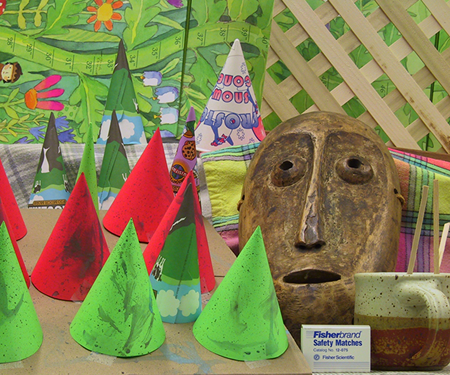
\includegraphics[width=0.33\textwidth]{figures/raw}
        \label{fig:images-raw}
    }
    \subfloat[LoG Transformation]{
        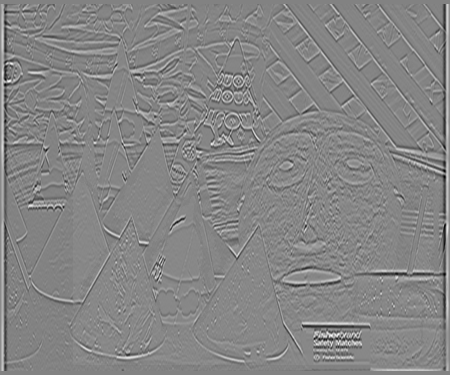
\includegraphics[width=0.33\textwidth]{figures/log}
        \label{fig:images-raw}
    }
    \subfloat[Disparity Map]{
        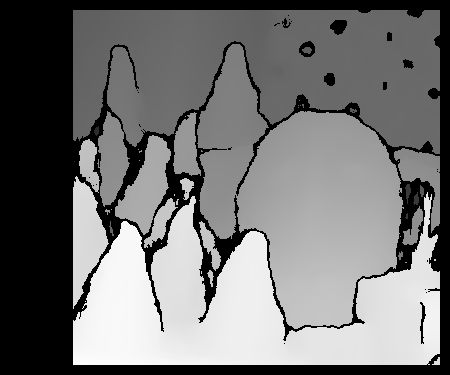
\includegraphics[width=0.33\textwidth]{figures/disparity}
        \label{fig:images-disp}
    }
    \caption{
        Left input image, output of the LoG transform, and the final disparity
        map after post-processing~\cite{konolige97}. This image is part of the
        Middlebury stereo dataset~\cite{scharstein2003}.
    }
    \label{fig:images}
\end{figure}

Rectification greatly reduces the number of pairwise comparisons that is
necessary and is a large performance boost, but na\"{i}vely calculating the SAD
between two windows still requires $\Theta(n^2)$ subtractions for a total
complexity of $\Theta(whDn^2)$. This performance can also be improved by
preprocessing the input images to generate one SAD integral image per possible
disparity. In general, the value of a pixel in an \textit{integral image} is
the sum of all pixels to the top-left of that pixel, inclusive. Given an
integral image, the area of an arbitrary rectangular region in the original can
be found in a constant number of operations. In this case, the integral is
computed from the horizontal components SAD errors shifted by the current
disparity. Assuming the disparity is $d$, the SAD integral image is recursively
defined as
\begin{align*}
    I_{sad}^{(d)}[x, y] =
        I_{sad}^{(d)}[x, y - 1]
        + \sum_{\Delta x = -n}^n
          \abs{I_l[x - \Delta x, y] - I_r[x - d - \Delta x, y]},
\end{align*}
where $I_{sad}^{(d)}[x, -1] = 0$ is the base case. This is simple to calculate
and has a time complexity of $\Theta(w h n)$.

From these integral images, generating the disparity is efficient. The
disparity $d$ and pixel $(x, y)$, the SAD error of this pair is simply
\begin{align*}
    \SAD(p, d) = I_{sad}^{(d)}[x, y + n] - I_{sad}^{(d)}[x, y - n]
\end{align*}
because of the properties of integral images. From this, the disparity of this
pixel is $I_{disp}[x, y] = \argmin_{d} \SAD(p, d)$, an operation that is
possible in $\Theta(D)$ time. This means that the entire disparity map can be
found in $\Theta(whD)$ time.

\begin{algorithm}[t]
    \KwIn {$I_l, I_r \in \mathbb{R}^{w \times h}$: rectified stereo pair}
    \KwIn {$n \in \mathbb{Z}$: half the width and height of the SAD window}
    \KwIn {$D \in \mathbb{N}_w$: maximum disparity}
    \KwOut {$I_{disp} \in \mathbb{N}_d^{w \times h}$: disparity map}
    $I_l^{(log)} \gets \LoG(I_l)$ \;
    $I_r^{(log)} \gets \LoG(I_r)$ \;
    %\STATE \COMMENT {compute vertical integral images of error}
    \For {$d = 1 \to D$} {
        \ForEach {$(x_0, y_0) \in \mathbb{N}_w \times \mathbb{N}_h$} {
            $E_y^{(d)} \gets \sum_{\Delta x = -n}^n \left(
                          I_l^{(log)}[x_0 - \Delta x, y_0]
                          - I_r^{(log)}[x_0 - \Delta x - d, y_0] \right)$ \;
            $I_{sad}^{(d)}[x, y] \gets E_y + I_{sad}^{(d)}[x, y - 1]$ \;
        }
    }
    %\STATE \COMMENT {choose the disparity for each pixel that minimizes error}
    \ForEach {$(x, y) \in \mathbb{N}_w \times \mathbb{N}_h$} {
        $I_{disp}[x, y] \gets \argmin_{d \le D} I_{sad}^{(d)}[x, y + n] - I_{sad}^{(d)}[x, y - n]$ \;
    }
    \Return {$I_{disp}$}
    \caption{Sum of Absolute Difference Block Matching (SAD-BM)}
    \label{alg:serial}
\end{algorithm}

While efficient, implementing the algorithm as described above would yield poor
disparity map simply because there is not enough texture in most images to
differentiate meaningful differences from noise. As in Konolige's
implementation ~\cite{konolige97}, this is solved by preprocessing the stereo
pair with the Laplacian of a Gaussian filter. The \textit{Laplacian of a
Gaussian} (LoG) is a convolution filter is a discrete approximation of the
composition of a Gaussian filter with the two-dimensional
Laplacian\footnote{The Laplacian is the sum of unmixed second-order partial
derivatives.}. This acts as a high pass filter that is robust to high-frequency
noise and ``amplifies'' texture. As can be seen in the difference between
\Cref{fig:images-raw,fig:images-disp}, LoG responds strongly to edges and
weakly to regions of constant color.

As LoG is a convolution filter it can be evaluated as a convolution in the time
domain or as multiplication in the frequency domain after taking the
discrete-time Fourier transform of the source images. While performing the
calculation in the frequency domain has better asymptotic complexity, it
performs poorly on small images. Therefore---as is typical in image
processing---the convolution will be directly evaluated using a ``sliding
window'' algorithm. This algorithm has a time complexity of $\Theta(whk^2)$
where $k$ is the width and height of the kernel. Because $k$ is constant
parameter\footnote{Typically $k$ is small because of precision limits when
discretizing the LoG function.}, this preprocessing step actually has a time
complexity of $\Theta(wh)$ and does not change the overall complexity.

This algorithm is summarized in \Cref{alg:serial} and has a total time
complexity of $\Theta(whDn)$ where $w \times h$ are the dimensions of the two
input images, $2n + 1 \times 2n + 1$ is the size of the SAD window, and $D$ is
the maximum disparity. With a sufficiently good implementation, a serial
version of this algorithm can process low resolution video in real-time.
However, achieving real-time processing at high resolutions or frame rates
requires a parallel implementation.

\section{Parallelization}
\label{sec:parallel}
Parallelizing the SAD-BM algorithm described in \Cref{sec:serial} is
challenging because of its several steps: (1) LoG filtering, (2) pre-computing
integral images, (3) error minimization. At a minimum, each of these steps must
be independently parallelized which requires a different technique for each
stage. Even worse, dependencies between the steps must be minimized or
worked-around to achieve optimal performance.

\subsection{OpenMP}
\label{sec:parallel-omp}
Modifying the serial algorithm to multiple threads is as easy as adding a few
OpenMP preprocessor directives. However, this comes at a steep cost: it is not
possible to intelligently ``pipeline'' the steps of the algorithm to maximize
CPU utilization. Even so, care must still be taken to avoid race conditions,
minimize thread overhead, and maximizing memory locality to get good cache
performance. In particular, achieving good cache performance requires careful
consideration of which nested loops should parallelized. 

First, consider the two-dimensional convolution required in the LoG
transformation. Assuming all images are stored in row-major order, this can be
done by assigning each thread a row, column, or single pixel. Given a
sufficient number of cores, assigning each pixel a thread would be ideal.
Unfortunately, modern CPUs have a small number of cores and the overhead of
creating this many threads would negate any performance gain from doing
multi-threading. Instead, the rows of the image will be partitioned into groups
of contiguous groups by OpenMP. This allows the number of threads to be tuned
to match the CPU's number of cores and guarantees that each thread will
sequentially accesses memory.

Once the LoG transformation is complete, the next step is to compute integral
images. Unlike with LoG, this cannot be done by partitioning the data into rows
because each row depends on all previous rows. One potential solution is to
partition the data into columns. Unfortunately, this splits sequential memory
accesses across threads and would not perform well on systems with a small
cache. This can be improved by spitting the calculation of integral images into
two steps: first partition the image into rows to compute the horizontal
component of the integral image, then sum along columns in parallel. This has
the same complexity of computing the integral in one pass, but minimizes the
number of non-sequential memory accesses.

Once the integral images have been pre-computed, the disparity of each pixel
can be independently computed and stored in the disparity map. For the same
reason as with LoG, the integral images will be partitioned into rows for this
calculation. Again, since each of these operations can be parallelized with no
additional synchronization. Each of these steps should have a linear speedup,
but the overall algorithm will still be subject to diminishing returns. This is
because of the unavoidable, constant overhead in waiting for threads to
synchronize between each step in the algorithm.

\subsection{NVIDIA CUDA}
\label{sec:parallel-cuda}
Unlike OpenMP's CPU threads, which are high overhead, parallelizing an
algorithm on a GPGPU with NVIDIA's CUDA architecture allows for massive
parallelism with zero-overhead threads and SIMD instructions.  However, this
performance comes at a cost: memory transfers between the CPU and GPU are very
slow and must be minimized at all costs ~\cite{cuda}. This means that the
stereo pair is transferred to the GPU as a single unit, all processing should
occur on the GPU, then the resulting disparity map is copied back to the CPU as
a single operation. In addition, care must be taken when choosing block sizes
to minimize the number of idle data paths in each CUDA core.

Once the stereo pair has been transferred to the GPU, LoG is very easy to
parallelize : each pixel in the image is assigned a thread and the entire
filtered image is generated in parallel. While this would be very inefficient
on the CPU because of the overhead of traditional threads, this is ideal for
the massively parallel architecture and zero-overhead threads available on the
GPU. Even with assigning one pixel per thread, it is still necessary to
partition the threads into blocks. For optimal performance the number of
threads per block must be a multiple of the warp size ~\cite{cuda}, $W$, which
is the number of SIMD data paths on each CUDA core. To minimize the number of
memory accesses---the slowest operation---per block, this was done by
partitioning the image into blocks of size $\floor{\sqrt{W}} \times
\floor{\sqrt{W}}$. This guarantees that memory accesses overlap as much as possible within each block and that each block contains approximately $W$ threads.

Once the LoG of both input images have been calculated, the next step is to
compute the integral images. This can be done using the same technique as
described in \Cref{sec:omp}; i.e. by first computing the horizontal SAD, then
summing along columns in the resulting image. Computing the horizontal SAD can
be done using square blocks of size $\floor{\sqrt{W}} \times \floor{\sqrt{W}}$
and the same partitioning scheme as described above. Summing the image
vertically cannot use this partitioning because rows are inter-dependent. Since
columns are independent, each column is assigned a thread and is grouped into a
block of size $1 \times W$. While less parallel than the other operations, this
is necessary to eliminate inter-thread communication.

Finally, the integral images are reduced to a disparity map using the same
algorithm as described in \Cref{sec:parallel-omp}. Just as with the LoG transformation,
each pixel is assigned a thread and is assigned to a $\floor{\sqrt{W}} \times
\floor{\sqrt{W}}$ block. Each pixel's thread finds the disparity that minimizes
SAD error as computed from the integral images. Once the disparity image has
been computed it either remains on the GPU for further CUDA-accelerated
operations or, more likely, is copied back to the host for manipulation on the
CPU.

\section{Performance Analysis}
\label{sec:perf}
The serial algorithm, OpenMP parallelized algorithm, and the CUDA parallelized
algorithm were each implemented in C++ using OpenCV data structures. In
addition, OpenCV was built with CUDA support so the open-source CPU and GPU
implementations of the algorithms could be evaluated. Each of these algorithms
was evaluated on the 2003 Middlebury stereo dataset and the results were
compared with ground truth to verify that each implementation was producing
valid output. Since the runtime of the algorithm is deterministic in the size
and bitdepth of the image it is only necessary to evaluate the algorithm on one
image and the \textit{cones} stereo pair from the
Middlebury~\cite{scharstein2003} dataset was arbitrary selected. The parameters
of SAD-BM were set to $D = 64$ and $n = 21$, values that are typical when the
tuned for real-time usage.

\begin{figure}
    \centering
    \subimport{figures/}{threads}
    \caption{
        Performance of the OpenMP algorithm evaluated on a machine with a 24
        cores, 800 MHz processor and a NVidia Teslda C2070 GPGPU. In
        \ref{fig:perf-omp} the number of threads is varied. Note the
        diminishing returns from Amdahl's law and the peak in performance at 24
        threads.
    }
    \label{fig:perf-omp}
\end{figure}

As \Cref{fig:perf-omp} shows, parallelizing SAD-BM with OpenMP performs as was
predicted in \Cref{sec:parallel-omp}: performance increases with the number of
threads until the number of threads exceeds the number of CPU cores. At this
point, performance slightly decreases due to the overhead of additional
threads.  While the parallel performance increase is impressive, it still
suffers from diminishing returns consistent with Amdahl's law, which states
that the maximum speedup of an algorithm is limited by the sections of the
algorithm that cannot be serialized. In this case, much of that overhead is
caused by splitting the algorithm into several smaller stages and could be
improved by pipelining the calculating so the stages can run in
parallel---something that is not possible with OpenMP (see \Cref{sec:future}
for details).

\begin{figure}
    \centering
    \subimport{figures/}{comparison}
    \caption{
        Comparison between algorithms described in this report and the open
        source implementations in OpenCV. Note that the GPU accelerated
        algorithms outperform their respective CPU algorithms and the OpenCV
        outperforms both of the custom implementations.
    }
    \label{fig:perf-comp}
\end{figure}

Overall, the OpenMP parallelization gave a large performance increase without
adding any complexity: parallelizing the serial algorithm with OpenMP only
required adding three preprocessor directives! Despite this boost in
performance, this algorithm runs 6.15 times slower than the OpenCV
implementation (\Cref{fig:perf-comp}). The impressive performance of OpenCV can
be attributed to three factors: (1) utilizing architecture-specific
instructions, (2) managing threads at a lower level, and (3) hand optimization
of inner loops.  In particular, OpenCV SAD-BM makes heavy use of Streaming SIMD
Extensions (SSE2) to perform multiple arithmetic operations in each clock
cycle. Combined with manually-controlled thread synchronization using Intel's
Thread Building Blocks (TBB) and loop unrolling, this easily accounts for the
performance difference.

Also as expected, the CUDA-accelerated SAD-BM algorithm is 2.71 times faster
than the OpenMP parallelized CPU algorithm. This is because the SAD-BM
algorithm---like many computer vision algorithms---is particularly well-suited
for massive parallelism. This speedup is lower than, but comparable to,
OpenCV's 7.37 times performance increase from the CPU and GPU algorithms. This
performance difference is harder to attribute, but is most likely from
intelligent use of CUDA streams and, similar to the CPU implementing, manual
loop unrolling. Using streams allow for more operations to be executed in
parallel, which is exceptionally important when working on powerful GPGPUs that
have a large number of CUDA cores such as the NVIDIA Tesla C2070 used for
performance evaluation.

\section{Conclusion}
\label{sec:conc}
Overall, the results (\Cref{fig:perf-comp}) show that parallelizing the SAD-BM
algorithm significantly improves performance. Using CPU threads on a multi-core
processor yields a considerable speedup without requiring expensive, additional
hardware or major changes to the serial algorithm. Indeed, running the
OpenMP-parallelized algorithm with one thread is exactly identical to running
the serial algorithm! Note, however, that this implementation is heavily
affected by the number of available CPU cores. While the performance is
excellent on a 24-core machine (such as that used for evaluation), it will
likely be disappointing on more common dual or quad core machines.

The ease of parallelizing SAD-BM with OpenMP is in contrast to the difficultly
in parallelizing the same algorithm with CUDA. Implementing the algorithm as a
collection of CUDA kernels required completely rewriting the serial algorithm
and carefully selecting optimal block sizes. The performance payoff, however,
is clear; if a high end GPGPU is available and performance is critical, then
GPU acceleration cannot be matched. Both of the CUDA-accelerated
implementations outperformed their corresponding multi-threaded CPU
implementations. This is especially important when the CPU is under heavy load
because any calculations done on the GPU free additional CPU time for other
tasks. One example of this would be for a mobile robot to offload stereo vision
calculations to its GPU while the CPU is responsible for path planning, a task
that does not lend itself to massive parallelism.

\section{Future Work}
\label{sec:future}
From the comparison with OpenCV, there are obviously improvements that would
improve the performance of both of the custom implementations. On the CPU this
would involve: (1) using SSE2 to perform multiple arithmetic calculations per
clock cycle, (2) manually unroll tight loops to reduce overhead, and (3)
switching to a lower-level threading library to reduce the amount of
synchronization. On modern processors, the SSE4.1 SIMD instructions for SAD
calculation could be used to even greater effect by allowing an $8 \times 8$
SAD window to calculated in less than eight clock cycles. These instructions
are not used in OpenCV, so this is a potential performance increase that could
surpass OpenCV's current speed.

Optimizations are less obvious on the GPU. Most importantly, the code should be
modified to use CUDA streams to pipeline operations and minimize the number of
synchronization points. Another major optimization would be to replace some
custom code, such as the LoG convolution, with algorithms from \textit{NVidia
Performance Primitives} (NPP), a highly optimized library of common algorithms.
At a lower level, performance could be improved by padding images to be a
multiple of the block size and manually unrolling loops to minimize bounds
checking in the kernels. Together, these improvements would close the gap
between the performance of these custom implementations of SAD-BM and the
highly optimized, open source implementations in OpenCV.

\bibliography{report}{}
\bibliographystyle{plain}

\end{document}
